\section{Introduction}%{Use Cases}
% looks odd to me not to have the first section titled "introduction"
\replace{%
    This document describes the planning for the evaluation activities in the \SUMMA project. The purpose of the evaluation is to test the functionality, efficiency, usefulness and user-friendliness of the components, technologies, integrated platform and use cases of the SUMMA platform and to provide feedback as part of the iterative development process.%
}{% with
    This document describes the methods and metrics that we will use to test the functionality, efficiency, usefulness, and user-friendliness of the technologies adapted for and developed within \SUMMA, the implementation of these technologies in actual software components, and the orchestration of these components within integrated web-based user interfaces. The results of these evaluations will provide valuable feedback to the developers as part of the iterative development process.%
}% end of replacement

In line with the Description of Action, \SUMMA will develop three use cases%
\ins{% moved here from below the list
. The first two were described in the report in Deliverable D1.1: \textit{Use Case Description and Requirements}. The third one will be developed in the course of the project. The three use cases are%
}% end of insertion
:

\begin{enumerate}
    \item External monitoring – intelligent tools to address the dramatically increased scale of the global news monitoring task;
    \item Internal monitoring – managing content creation across several languages;
    \item Data journalism – \replace{using}{augmenting} the \SUMMA platform \replace{to graphically visualise}{with visualisation tools for} some of the \replace{measurable}{quantitative} \SUMMA output.
\end{enumerate}

\cut{%moved up before the enumeration
The first two use cases have been described in deliverable D1.1 (Use Case Description and Requirements). The third one, on Data Journalism, will be developed in the course of the project. The internal and external use cases use the same underlying system and will primarily differ in terms of filtering and dashboarding options. 
}% end of cut

The \SUMMA \replace{tool}{platform prototype, to be released in Month 15,} provides a common \replace{platform}{framework} for the \ins{first} three \cut{primary} use cases\cut{, i.e., internal and external monitoring}.
\ins{Many of the evaluation aspects will thus be similar, but their \replace{importance}{relevance for the respective use case} may differ.}
\ins{At a later stage of the project, }\replace{This}{the} \ins{basic} platform will be enhanced with a customised dashboard\cut{ at a later stage of the project}.
\replace{The main functionalities are common to both use cases. Therefore, many of the evaluation aspects will be similar, although the importance may differ. In year 3, the}{This} dashboard customisation will be evaluated \ins{in Year 3}.

% \UG{Consider adding a brief general document outline paragraph here. - done, but inserted in the abstract instead}

\begin{figure}[ht]
    \centering
    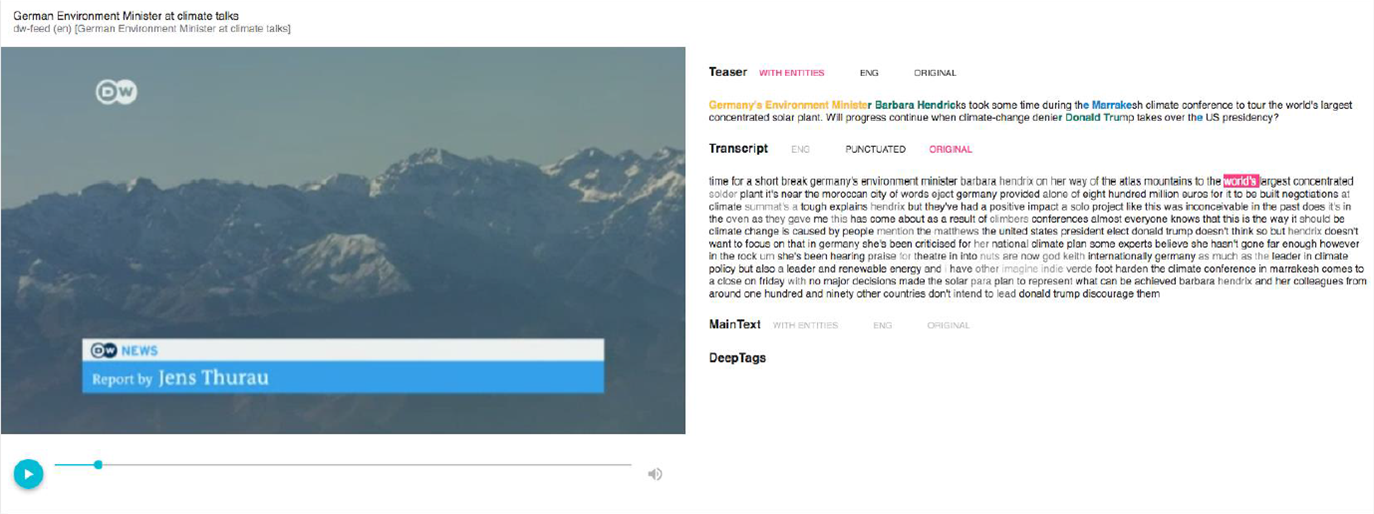
\includegraphics[width=1.0\textwidth]{./images/SUMMA_platform_2016.png}
    \caption{\SUMMA User Interface (prototype)}
    \label{fig:SUMMA platform}
\end{figure}